\title{DRAFT: Measuring a Block and a Cylinder}
\author{Jason Press}

\documentclass{article}

\usepackage{setspace}
\usepackage{mathtools}
\usepackage{graphicx}

\DeclareGraphicsExtensions{.jpeg}


\begin{document}

\maketitle

\begin{abstract}

	No tool is infinitely precise. There is a certain amount of variability associated with making a measurement with any tool. In this lab, we measured the volume of a wooden block and a cylinder, and used the error propagation formula to determine the range of the true volume of the two objects. This was done for three measuring devices: a roll tape measure, a ruler, and a set of precision calipers. As more precise tools were used, the amount of error became smaller.

\end{abstract}

% \doublespacing


\section{Introduction}

The aim of this lab was to measure the volume of two objects: a block, and a cylinder. To obtain the volume of the objects, three different measurement tools were used: a roll tape measure, a ruler, and precision calipers. However, the volume has to have upper and lower bounds, since the measuring tools have upper and lower bounds and do not have infinite precision: the measuring tools have an upper and lower bound of precision.

To measure the volume of the block, three measurements were taken: length, width, and height. If those quantities are known, the volume of a rectangular prism can be precisely calculated as $V_{prism}=LWH$. However, since the measuring tools are not perfect, the volume has to be calculated as $V_{block}=LWH+\sigma_{V}$, where $\sigma_{V}$ is the error due to the measuring tools being not infinitely precise and accurate. Similarly, for the cylinder, two measurements were taken: diameter and height. Using similar logic, but with the formula for a circle, the volume of a cylinder has to be similarly calculated as $V_{cylinder}=\pi R^{2}H + \sigma_{V}=\pi (\frac{D}{2})^{2}H+\sigma_{V}$.

In general, $\sigma_{V}= \sqrt{\sum_{L} \frac{\partial V}{\partial L}^{2}\sigma_{L}^{2}}$ for all measurements $L$, where $\sigma_{L}=\sqrt{\sigma_{sys,L}^{2}+\sigma_{res,L}^{2}+\sigma_{stat,L}^{2}}$ for some measurement $L$. This is the sum of the main categories of errors in all measurements. $\sigma_{stat,L}$ is assumed to be zero, since repeated measurements with a given device yield the same result; $\sigma_{res,L}$ is half the resolution of the measurement device; and our group assumed $\sigma_{sys,L}$ to be equal to $\sigma_{res,L}$, since that seemed to be about right for any error that could be caused by a misread of the measuring device or any other reasonable systematic error. Like $\sigma_{V}$, $\sigma_{L}$ is the sum of the main categories of errors, but for a specific measurement $L$. Because we assume $\sigma_{res,L}=\sigma_{sys,L}$ for this experiment, $\sigma_{L}=\sqrt{2\sigma_{res,L}^{2}}$.

\section{Methods}

The tools used in this lab were a roll tape measure, a ruler, and a set of precision calipers. The objects measured by the tools in this lab were a friction block and a metal cylindrical weight. Although optional, a tabletop makes using the measuring devices easier, and was used in this lab.

For measuring with the roll tape measure and the ruler, one end of the quantity to be measured was placed on a convenient marking, such as the 20cm mark. Then, while keeping the end on the aforementioned mark, the edge was carefully aligned with the object to get the most accurate representation of length. Finally, the end point was recorded, rounded to the nearest tick mark. See Figure~\ref{fig:ruler-block} for a visual representation.

For the diameter of the cylinder, there was a center point marked with a threaded hole. Instead of the edge of the measuring device running along a defined edge, the edge was ran through the threaded hole to make a line through the center of the base circle, ensuring the true diameter length was measured. See Figure~\ref{fig:ruler-cylinder} for a visual representation.

For the calipers, the desired dimension was placed along the flat edge of the calipers. Then, a reasonable amount of pressure was applied to the calipers so the object would not distort, but not slip. Then, the number was recorded.

\begin{figure}[!htbp]
	\centering
	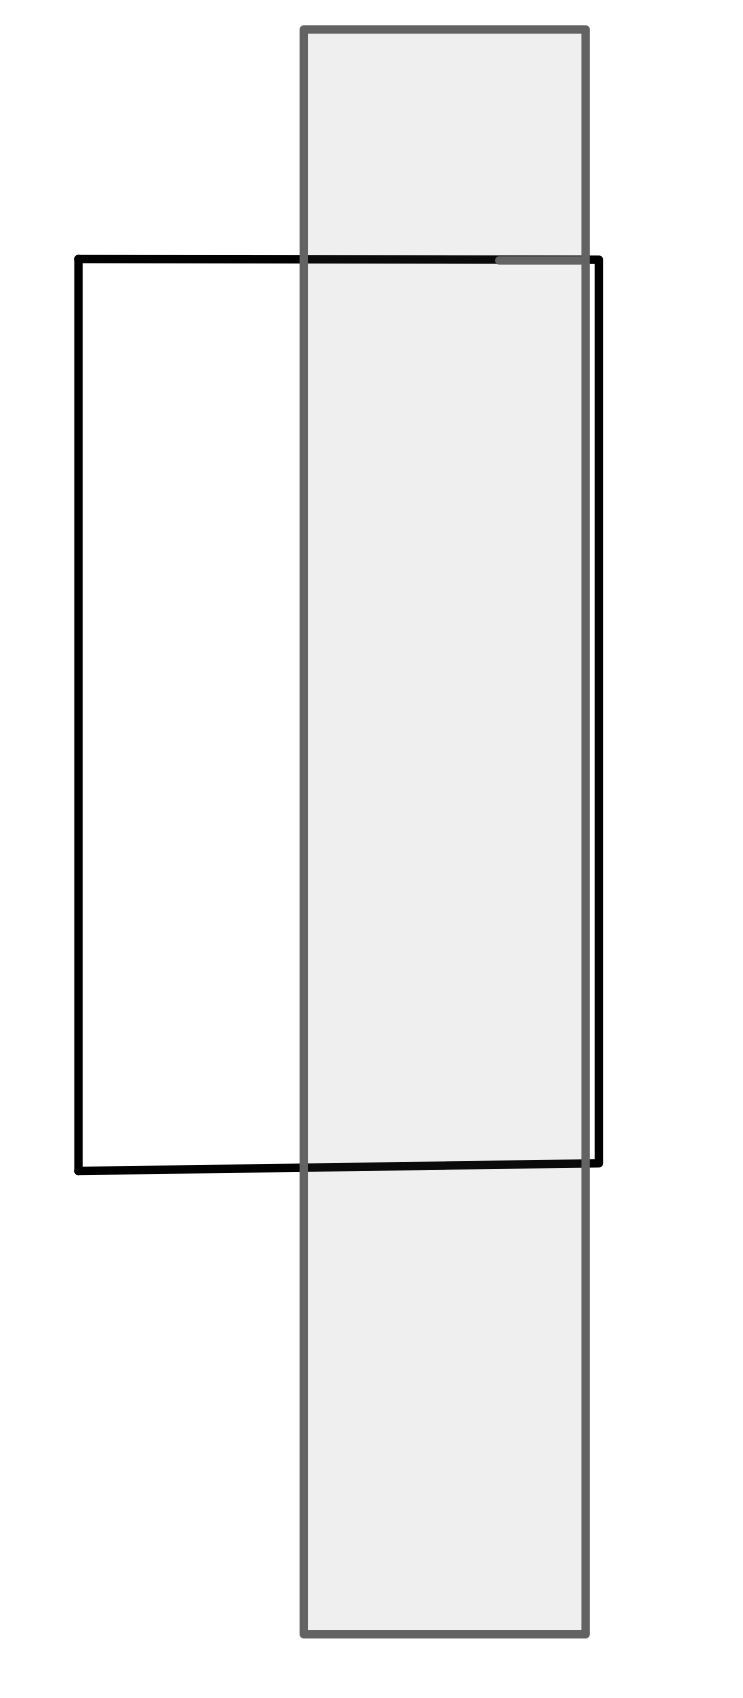
\includegraphics[totalheight=8cm]{IMG_0621.jpeg}
	\caption{Using a ruler (in gray) to measure the edge of block (in black).}
	\label{fig:ruler-block}
\end{figure}

\begin{figure}[!htbp]
	\centering
	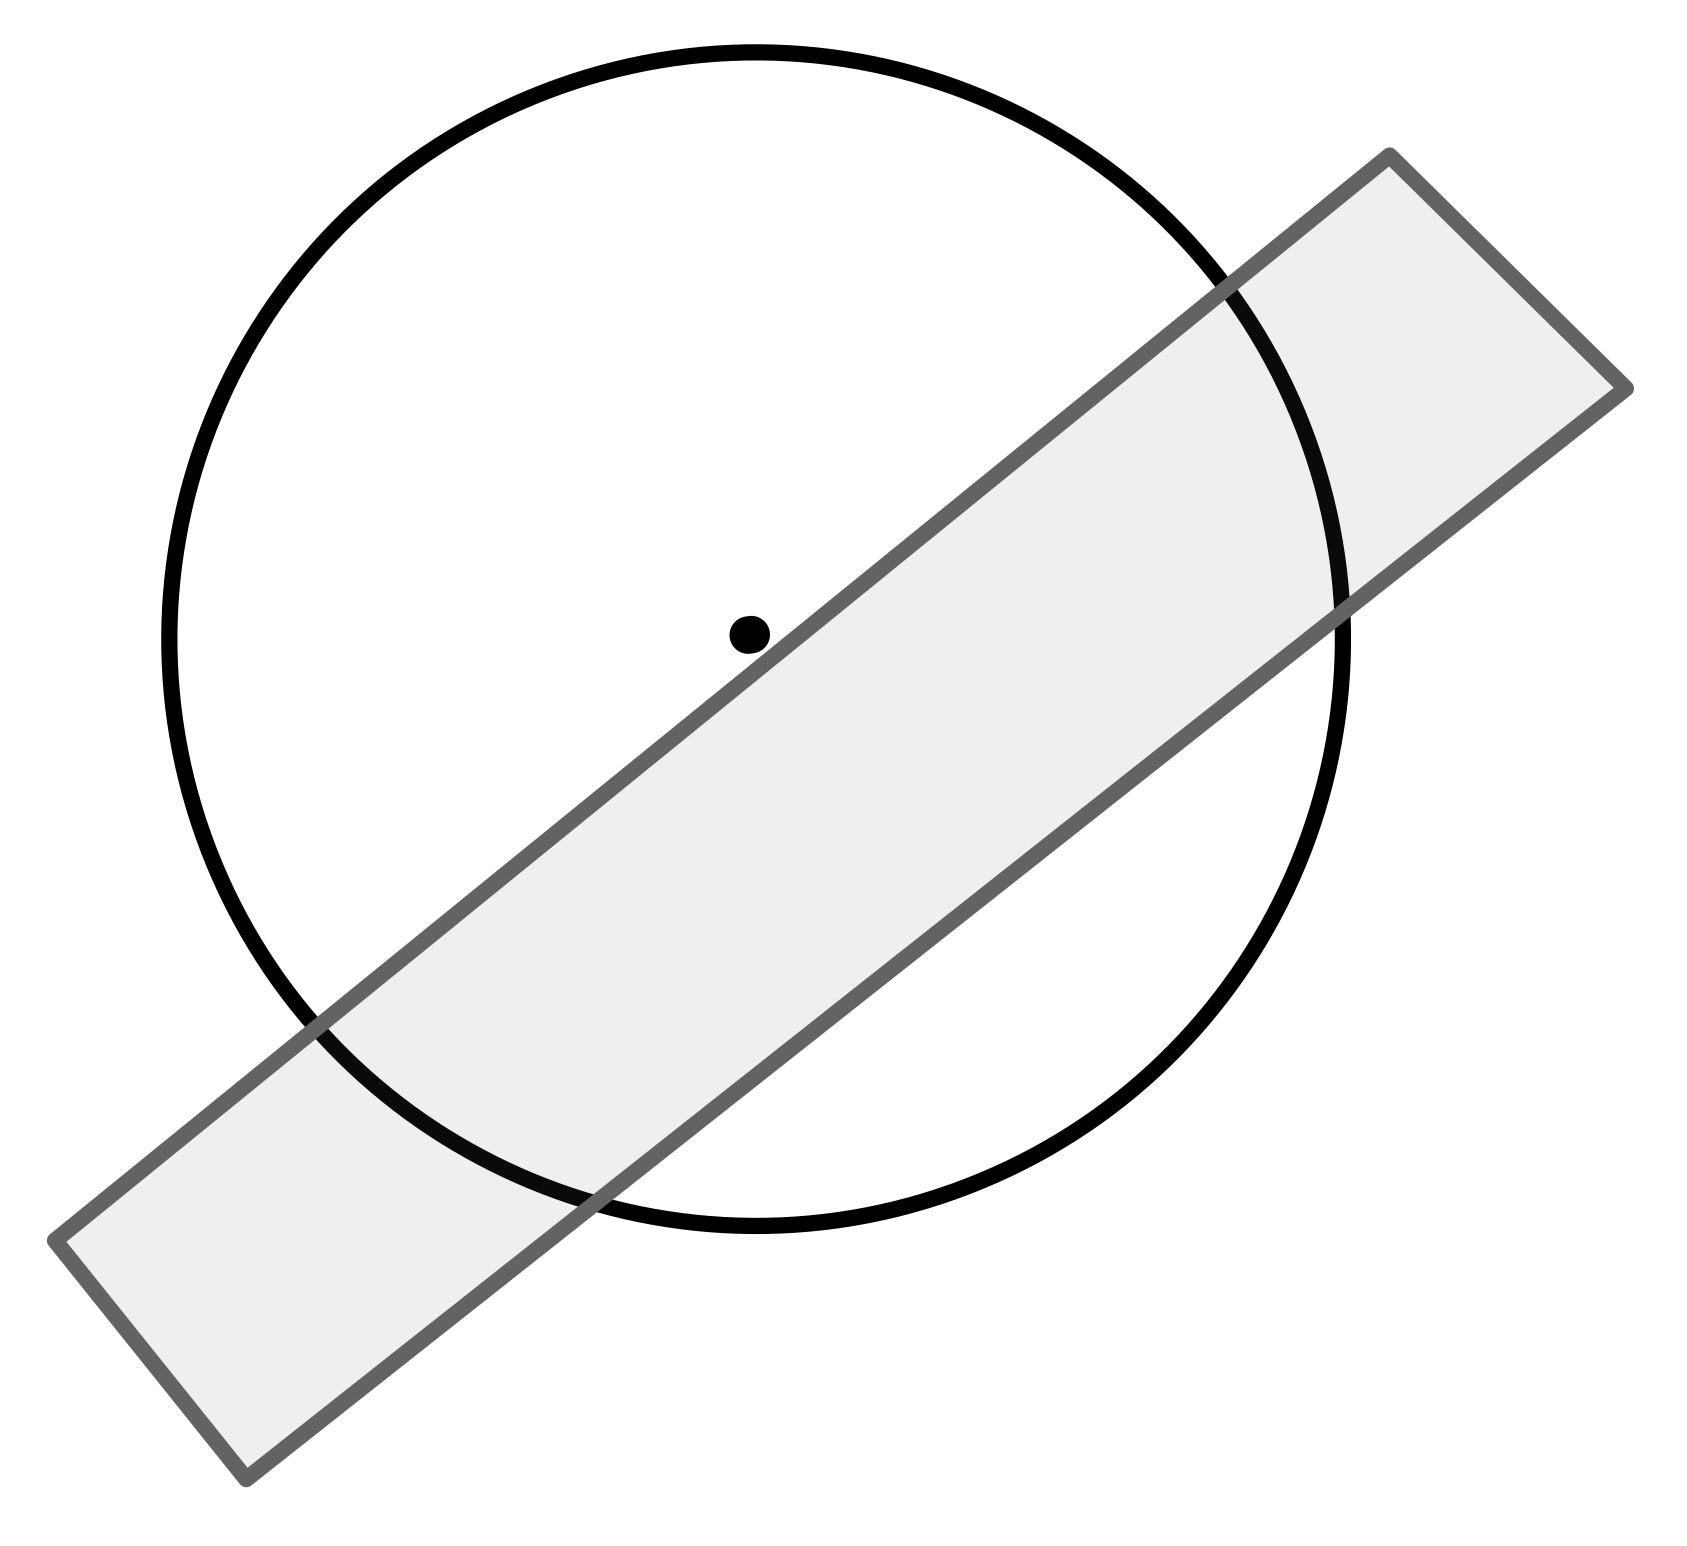
\includegraphics[totalheight=6cm]{IMG_0623.jpeg}
	\caption{Using a ruler (in gray) to measure the diameter of the cylinder (in black) through the center dot.}
	\label{fig:ruler-cylinder}
\end{figure}


\section{Results}

These are the results of the measurements of the respective objects, along with the resolution of the device.

\begin{table}[!htbp]
	\centering
	\begin{tabular}{lllll}
		          & Length & Width & Height & Resolution \\
		Roll Tape & 2.6    & 5.2   & 13.2   & 0.2        \\
		Ruler     & 2.7    & 5.2   & 13.2   & 0.1        \\
		Calipers  & 2.644  & 5.131 & 13.145 & 0.001
	\end{tabular}
	\caption{Measurements for the block, in cm.}
	\label{block-table}
\end{table}

\begin{table}[!htbp]
	\centering
	\begin{tabular}{llll}
		          & Diameter & Height & Resolution \\
		Roll Tape & 2.6      & 7.6    & 0.2        \\
		Ruler     & 2.5      & 7.6    & 0.1        \\
		Calipers  & 2.540    & 7.610  & 0.001
	\end{tabular}
	\caption{Measurements for the cylinder, in cm.}
	\label{cylinder-table}
\end{table}

These are the results of the calculated volumes, with the attached error propagation.

\begin{table}[!htbp]
	\begin{tabular}{lll}
		          & Block                   & Cylinder          \\
		Roll Tape & $1.7\times10^{2}\pm11$  & $40\pm4.4$        \\
		Ruler     & $1.9\times10^{2}\pm5.6$ & $37\pm2.1$        \\
		Calipers  & $178.3\pm0.05450$       & $38.56\pm0.02177$
	\end{tabular}
	\caption{Calculated volumes with error propagation, in cm$^3$.}
	\label{volume-table}
\end{table}

As Table~\ref{volume-table} demonstrates, as the resolution of the instrument becomes smaller, the error propagation decreases.

\section{Discussion}

Ultimately, the purpose of this lab is to get used to working in a laboratory enviornment: to get used to handling equipment, telling lab partners what to do, recording measurements, and making a lab report. Yes, there is value in measuring the objects, but no relevant information was gained by doing so, because the precise volume of the block and cylinder is more or less irrelevant.

For any resolution $r$, the expected $\sigma_{r}$ is $\sqrt{2(\frac{r}{2})^{2}}$. As tools get more precise, i.e. $\lim\limits_{r \to 0}=0$, the amount of error propagation also approaches zero, i.e. $\lim\limits_{r \to 0} \sigma_{r} = \lim\limits_{r \to 0} \sqrt{2(\frac{r}{2})^{2}}=0$. This theory is reflected practically with the observed error propagation decreasing with more precise tools.

The amount of statistical error in this lab is roughly zero. This is reflected with all measurements being roughly equal, within a reasonable margin of error. For example, in Table \ref{block-table}, all length measurements are within half of the resolution of the available tools, i.e. $2.6\pm0.1 \approx 2.7\pm0.05 \approx 2.644\pm0.0005$. Unless all three tools are equally off by the same amount, which is very unlikely, this fact alludes to a negligable amount of statistical error.

The amount of systematic error in this lab is an overestimate of what it reasonably should be. Having three people agree that the measurement was correct is a lot more confident than just one person. It was agreed that the amount of systematic error in the experiment would be at most equal to the resolution error, so out of an abundance of caution, the amount of systematic error was chosen to be equal to the amount of resolution error.

\section{Sample Calculations}

All calculations were done by hand. To demonstrate what calculations were used, here is how the volume of the cylinder recorded by the ruler was calculated. All measurements are from Table~\ref{cylinder-table}.

$$
	\\
	R = \frac{2.5}{2}= 1.25 \\

	\sigma_{ruler} = \sqrt{2\sigma_{res,ruler}^{2}} = \sqrt{2 \left( \frac{0.1}{2} \right) ^{2}}=0.0707 \text{cm} \\

	\sigma_{V} = \sqrt{\sum_{L} \frac{\partial V}{\partial L}^{2}\sigma_{L}^{2}} = \sqrt{\left(\pi R H\right) ^{2}\sigma_{ruler}^{2} + \left( \pi R^{2} \right) ^{2}\sigma_{ruler}^{2}} \\

	\sigma_V=\sqrt{\left(\pi(7.6)(1.25)\right)^20.0707^2 + \left(\pi R^2\right)^2 0.0707^2}=2.13 \text{cm}^3 \\

	V_{cylinder} = \pi R^{2}H + \sigma_{V} = \pi (\frac{D}{2})^{2}H+\sigma_{V} \\

	V_{cylinder} = \pi (1.25)^2 (7.6) + 0.0707 = 37 \pm 2.1 \text{cm}
$$


\end{document}
